\documentclass[article, 11pt]{IEEEtran}   %Document is an article, 11 pt font, and follows IEEE format
\usepackage{hyperref}         %Use hyperref package (for hyperlinks)
\usepackage{graphicx}         %Use graphicx package (for images)
\usepackage{float}            %Use float package (allows you to place images more easily)

\usepackage{gensymb}          %Use gensymb package (generic symbols)
\usepackage{amsmath}          %Use amsmath package (for optimized math formulas)
\usepackage{tikz}             %Use tikz package (for creating graphics)
\usepackage{pgfplots}         %Use pgfplots package (for creating graphics)
\usepackage{pgfplotstable}    %Use pgfplotstable (for linear regression)
\usepackage[spanish]{babel}


\begin{document}
%
% paper title
% Titles are generally capitalized except for words such as a, an, and, as,
% at, but, by, for, in, nor, of, on, or, the, to and up, which are usually
% not capitalized unless they are the first or last word of the title.
% Linebreaks \\ can be used within to get better formatting as desired.
% Do not put math or special symbols in the title.
\title{Proyecto 1\\Aplicaciones de EDO}

% author names and affiliations
% use a multiple column layout for up to three different
% affiliations
\author{
	\IEEEauthorblockN{Juan José Rivera Román - 20002802}
	\IEEEauthorblockA{\\Universidad Galileo\\Guatemala, Guatemala }
}

% make the title area
\maketitle

% As a general rule, do not put math, special symbols or citations in the abstract
\begin{abstract}
Uno Esta secci\'on es un breve resumen de los aspectos m\'as importantes del reporte. Se incluye el pr\'oposito del laboratorio, los hallazgos m\'as importantes y la conclusi\'on principal.
\end{abstract}

\section{Introducci\'on}
En esta secci\'on se establece el objetivo del laboratorio. La introducci\'on debe incluir la siguiente informaci\'on:
\begin{itemize}
	\item Contexto de aprendizaje del laboratorio.
	\item Los objetivo principales.
	\item Hip\'otesis que se desea confirmar o rechazar,debe incluir el razonamiento.
\end{itemize}
 
\section{Procedimiento}
Un breve resumen del procedimiento utilizado en la pr\'actica.

\subsection{Materiales}
Materiales utilizados f\'isico o digital
\begin{itemize}       							%Creating an unordered list
\item Computadora modelo, hardware relevante de la computadora que fue necesario para la implementaci\'on
\item Software
\item Base de datos [referencia]
\end{itemize}

\subsection{Diagrama de configuraci\'on del laboratorio}
Incluye diagrama de la configuraci\'on o la forma en que se elaboro el experimento. Por ejemplo, la configuraci\'on en la que se conecto el equipo con el que se hizo alguna medici\'on. 

\begin{figure}[H]									%Creating a figure with caption
\centering
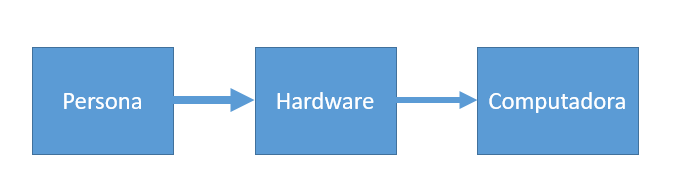
\includegraphics[scale=0.7]{conf}%Inserting graphic file (in same directory)
\caption{Ejemplo de la configuraci\'on de un Sistema}\label{diagram1}  %Captioning the graphic file
\end{figure}

\subsection{Pasos del procedimiento}        		
Se enumeran los pasos realizados para obtener los resultados. 
\begin{enumerate}						%Creating an ordered list
	\item Paso 1
	\item Paso 2
	\item Paso 3
\end{enumerate}

\section {Resultados}
Esta secci\'on incluye \'unicamente los resultados obtenidos. Estos se pueden presentar en forma de tablas o gr\'aficas dependiendo del tipo de informaci\'on que se obtenga.

\subsection{Tabla de datos}
\begin{table}[H]
\centering
\caption{Ejemplo de Tabla con datos}
\label{DataTable1}
\begin{tabular}{|c|c|}
\hline
Diameter (cm) & Circumference (cm) \\
\hline
11.7 & 37.8\\
17.1 & 54\\  
8.4 & 26.6\\
6.6 & 21.2\\
7.4 & 23.4\\
6.6 & 21.2\\
7.9 & 25.6\\
15.8 & 50.6\\
8.8 & 28.5\\
1.9 & 7\\
\hline   
\end{tabular}
\end{table}
\newpage

\subsection{Graficas}
\begin{figure}[H]
\centering
\begin{tikzpicture}
\begin{axis}[
   title=Scatterplot of Circle Quantities,	%Title of graph
   xlabel={diameter (cm)},					%label the x-axis
   ylabel={circumference (cm)},				%label the y-axis
   legend pos=south east,					%put slope legend in bottom right corner
]
\addplot[blue, only marks] table {CircleData.dat};	%plot points from data table
\addplot [red] table [y={create col/linear regression={y=y}}]   %best fit line
        {CircleData.dat};
       
\addlegendentry{slope=$\pgfmathprintnumber{\pgfplotstableregressiona}$}        
        %show slope value
\end{axis}
\end{tikzpicture}
\caption{Ejemplo de gr\'afica}\label{diagram1}   %caption the graph
\end{figure}

\section{Discusi\'on / An\'alisis}
En esta secci\'on se discute los resultados obtenidos en el laboratorio. Esta incluye la interpretaci\'on de los datos, el an\'alisis y explicaci\'on de los resultados . \textbf{Esta es la parte m\'as importante del reporte}

\section{Conclusi\'on}
Esta secci\'on incluye una \'ultima discusi\'on de los resultados y como estos se relacionan con la hip\'otesis descrita en la introducci\'on.
La idea es transmitir lo que se ha aprendido al realizar la pr\'actica.\\ \\
En las referencias se incluyen toda la bibliograf\'ia utilizada, as\'i como las fuentes de donde se obtuvo la data.
%FORMATO APA
\begin{thebibliography}{1}

\bibitem{LabWrite}
M.~Carter, E.~Weiebe, and M.~Ferzli, \emph{LabWrite}, \url{https://www.ncsu.edu/labwrite/index_labwrite.htm}, NC~State~University, 2004.

\bibitem{Fullerton}
D.~Fullerton, \emph{APlusPhysics}, \url{http://www.aplusphysics.com/courses/regents/lab_report.html}, 2016.

\bibitem{Svoronos}
T.~Svoronos, \emph{How I Will Write My Dissertation}, \url{http://teddysvoronos.com/2014/12/26/how-i-will-write-my-dissertation-3/}, 2014.

\bibitem{Clarion}
G. Clarion, \emph{Rocklin High School}, 2009.

\end{thebibliography}

\end{document}